\documentclass[border=4pt,tikz]{standalone}
\usepackage[utf8]{inputenc}
\usepackage[T1]{fontenc}
\usepackage{tikz}
\usepackage{xcolor}
\usetikzlibrary{positioning, arrows.meta, calc}
\definecolor{nodeFill}{HTML}{E8EEF7}
\definecolor{nodeStroke}{HTML}{1F3A5F}
\definecolor{accent}{HTML}{3D5A80}
\definecolor{soft}{HTML}{F4F1EA}
\definecolor{softStroke}{HTML}{8B7355}
\definecolor{textDark}{HTML}{1A1A1A}
\begin{document}
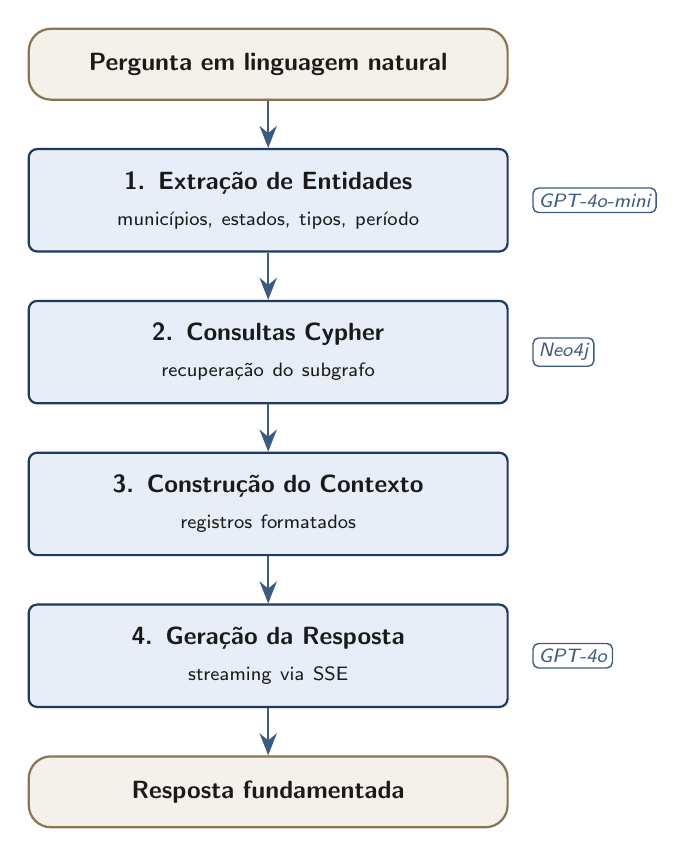
\begin{tikzpicture}[
  font=\sffamily\small,
  every node/.style={text=textDark},
  io/.style={
    rectangle, rounded corners=8pt,
    draw=softStroke, line width=0.8pt, fill=soft,
    text width=58mm, minimum height=9mm,
    align=center, inner sep=4pt
  },
  stepbox/.style={
    rectangle, rounded corners=3pt,
    draw=nodeStroke, line width=0.8pt, fill=nodeFill,
    text width=58mm, minimum height=13mm,
    align=center, inner sep=4pt
  },
  techbadge/.style={
    rectangle, rounded corners=2pt,
    draw=accent, line width=0.5pt, fill=white,
    font=\sffamily\scriptsize\itshape,
    text=accent, inner sep=2pt
  },
  flow/.style={
    -{Stealth[length=2.8mm, width=2.2mm]},
    draw=accent, line width=0.8pt
  }
]
  \node[io] (input) {\textbf{Pergunta em linguagem natural}};

  \node[stepbox, below=6mm of input] (extract)
    {\textbf{1. Extração de Entidades}\\[2pt]
     \scriptsize municípios, estados, tipos, período};
  \node[techbadge, right=3mm of extract] {GPT-4o-mini};

  \node[stepbox, below=6mm of extract] (cypher)
    {\textbf{2. Consultas Cypher}\\[2pt]
     \scriptsize recuperação do subgrafo};
  \node[techbadge, right=3mm of cypher] {Neo4j};

  \node[stepbox, below=6mm of cypher] (context)
    {\textbf{3. Construção do Contexto}\\[2pt]
     \scriptsize registros formatados};

  \node[stepbox, below=6mm of context] (gen)
    {\textbf{4. Geração da Resposta}\\[2pt]
     \scriptsize streaming via SSE};
  \node[techbadge, right=3mm of gen] {GPT-4o};

  \node[io, below=6mm of gen] (output) {\textbf{Resposta fundamentada}};

  \draw[flow] (input)   -- (extract);
  \draw[flow] (extract) -- (cypher);
  \draw[flow] (cypher)  -- (context);
  \draw[flow] (context) -- (gen);
  \draw[flow] (gen)     -- (output);
\end{tikzpicture}
\end{document}
